\textbf{Входные параметры:}

 x --- переменная.

\textbf{Возвращаемое значение:}
 
 Значение функции Хевисайда.
 
\textbf{Формула:}
\begin{equation*}
F\left(x \right)=\left\lbrace \begin{aligned}
1&\text{, если } x>0; \\
0&\text{, если } x\leq 0.
\end{aligned}\right. 
\end{equation*}

 \begin{figure} [h] 
   \center
   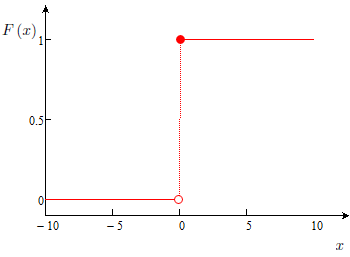
\includegraphics {TMHL_HeavisideFunction_Graph.png}
   \caption{График функции} 
   \label{img:TMHL_HeavisideFunction_Graph}  
 \end{figure}
 
